\subsection{Incremental LSTM-based Dialog State Tracker \cite{Zilka2015}}

A dialog state tracker estimates the user's goal throughout the dialog by analyzing the \emph{automatic speech recognition (ASR)} outputs for the user's utterance. This paper presents an incremental dialog state tracker based on LSTM networks. It directly uses ASR hypothesis to track the state.

Because of uncertainty in the user input, statistical dialog systems maintain a distribution over all possible states, called the belief state. In this paper, a dialog state at time $t$ is defined as a vector $s_t \in C_1 \times ... \times C_k$ of $k$ dialog state components (sometimes also called slots). Each component $c_i \in C_i = \{ v_1, ..., v_{n_i} \}$ takes one of $n_i$ values. The goal of the dialog state tracker is to give the probability distribution over one of the independent components $p(c_i | w_1, ..., w_t)$.

\begin{figure}[h]
  \centering
  % Requires \usepackage{graphicx}
  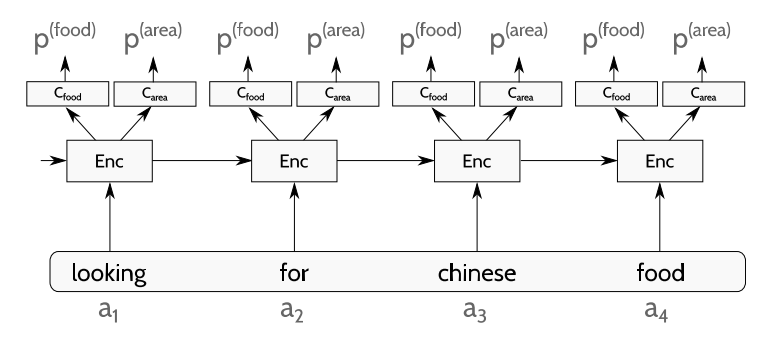
\includegraphics[width=.7\linewidth]{11_28_dstc_ilstm.png}\\
  \caption{A demonstration of the proposed model}\label{fig:dstc_ilstm}
\end{figure}

The main idea of this paper is to use LSTM to encode the information from the input word sequence into a fixed-length vector representation. Given this representation, a classifier returns a probability distribution over the value of the dialog state. An example of the model applied to a particular input sentence is at Figure \ref{fig:dstc_ilstm}.

Formally, the input neural network maps the word $a$ and its ASR confidence score $r$ to a joint representation $u$: $u = NN(a, r)$. The representation $u$ is used by the LSTM encoder along with the previous hidden state $q_{t-1} = (c_{t-1}, h_{t-1}$ to create a new hidden state $q_t$: $q_t = Enc(u, q_{t-1})$. The classifier, represented by a single softmax layer, then maps the hidden state to a probability distribution over all possible values: $p_t = C(h_t)$.

The training criterion is a cross-entropy loss for a dialog example, which is annotated by true labels at some points in time:
$$l(\theta) = - \sum_{t \in Y} \log LecTrack(a_1, r_1, ..., a_n, r_n)_{y_t}^t,$$
where $y_i$ denotes a label for the dialog state at time $i$, and $Y$ is a set of times where the label $y_i$ exists.

In the experimental study, the paper shows that the propose model yields performance to the state-of-the-art system. For example in the requested component, the proposed method achieves 0.98 accuracy and 0.04 L2 score, which is identical to the result of the previous best system. 